\chapter{Инженерная часть: Проектирование и Реализация ПО}

Для простоты считаем что решаемая задача заключается в классификации изображений на 10 классов (по аналогии c задачей CIFAR-10 по отношению к ImageNet)
В связи с этим многие элементы системы могут быть упрощены:
В частности нет необходимости описывать подробно работу с пространственным разбиением.
\section{Проектирование системы геолокации по серии изображений}

\begin{figure}[h]
	\centering
	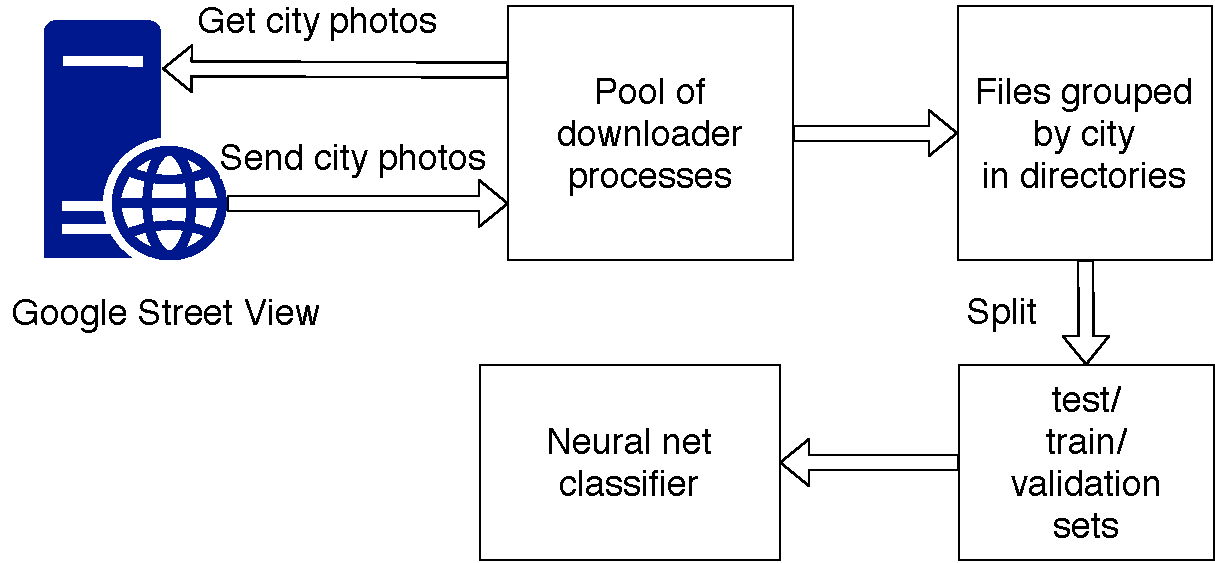
\includegraphics[width=0.7\linewidth]{img/dataset_generation}
	\caption{Схема для генерации датасета}
	\label{fig:datasetgeneration}
\end{figure}

Опишем на высоком уровне работу системы:
Мы собираем датасет из панорам \texttt{Google Street View} в 10 городах, определённых своими координатами. Запросы в \texttt{API} выполняются параллельно пулом из 4 процессов, которые раскладывают изображения в директории соответствующие классам. Эти 10 классов можно заменить $ K $
\texttt{S2}- ячейками и набирать из каждой ячейки фотографии с другого сервиса, такого как Flickr (см \cite{im2gps}). Для 10 классов можно набрать по 100 представителей каждого класса.

После этого мы разбиваем этот набор в соотношении $ 8,1,1 $
обучающая, тестовая, валидационная выборки, после чего приводим структуру файлов к формату, который понимает функция \texttt{torchvision.datasets.ImageFolder}, а именно: кладём фотографии в директории, соответствующие фазе обработки (train, test, val).

Этот процесс показан на рисунке \ref{fig:datasetgeneration}

Так как мы используем нейросетевые методы имеет смысл использовать модель классификации end-to-end, то есть:
$ y = CLS(x) $, где $ x $ --- фотография, нормированная для улучшения процесса классификации, $ y $ --- класс, относимый сетью этой фотографии.

Для реализации этой модели мы воспользуемся предобученными моделями из программного пакета \texttt{torchvision},
также предоставляющего нормирующие преобразования, функции аугментации данных (для расширения обучающей выборки), потокового чтения данных.

\section{Архитектура подсистемы классификации}

Из доступных предобученных моделей выберем несколько подходящих под следующие критерии:
\begin{itemize}
\item параметры полностью помещаются в память GPU автора (4GB), что необходимо для обучения/дообучения;
\item архитектура позволяет дообучать модель;
\item сеть демонстрирует точность выше $ 0.8 $ на датасете ImageNet.
\end{itemize}
Таким критериям отвечают:
resNet34, resNet50, squeezeNet, Inception\_V3, DenseNet.

Все эти сети являются глубокими свёрточными нейросетями, а потому подробное рассмотрение внутреннего устройства и теоретических преимуществ функционирования помимо описанных в Разделе \ref{chapter2} выходит за рамки данной работы.

Благодаря модульности и динамичности пакета \texttt{pytorch}, обучающий алгоритм и алгоритм визуализации не зависят от используемой архитектуры сети.

Оценивать точность будем при помощи \texttt{sklearn.metrics} содержащего реализации помимо прочего процедур вычисления $ F1 $-меры, матрицы неточностей, отчёта о классификации; и пакета \texttt{torch.nn}, реализующего функцию потерь перекрёстной энтропии и множество нейросетевых примитивов, таких как: полносвязные и свёрточные слои, SoftMax, Pooling и различные нелинейности.

\section{Взаидодействие с моделью}

Библиотека предоставляет возможность сериализации модели что позволяет переисользовать 
исследовательский прототип в приложениях. Так можно обучить модель и затем встроить её в 
более крупную систему, такую как веб или мобильное приложение. 

Взаимодействие с исследовательским прототипом осуществляется с помощью механизмов интерактивных рабочих тетрадей \texttt{Jupyter Notebook}.

\begin{figure}[h]
	\centering
	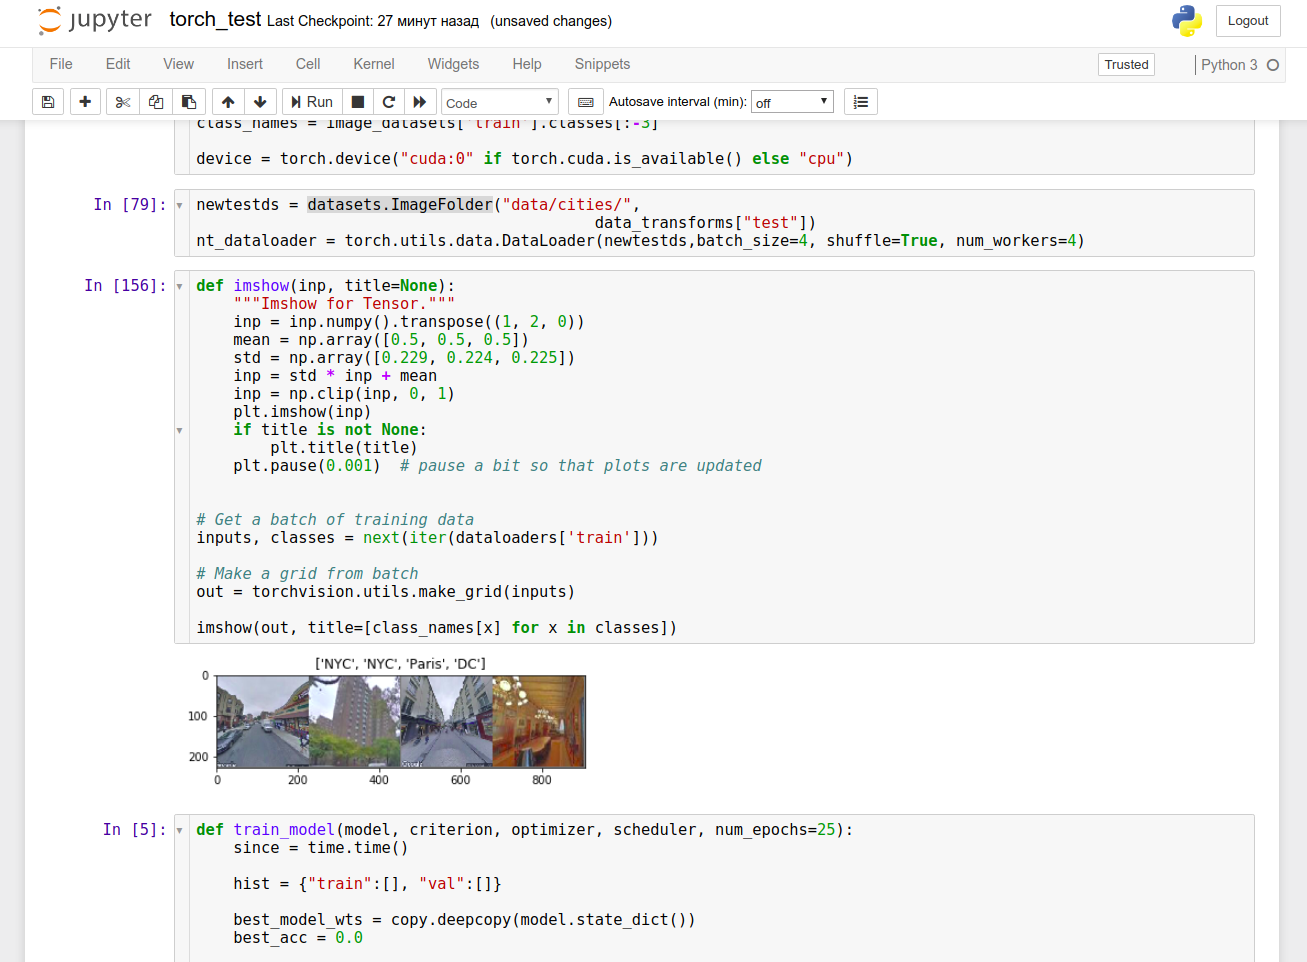
\includegraphics[width=0.7\linewidth]{img/notebook}
	\caption{интерактиная рабочая тетрадь jupyter}
	\label{fig:notebook}
\end{figure}


\section{Выводы}

Были разработаны модули генерации датасета, разбиения на обучающую/тестовую выборки и 
классификации. Были реализованы процедуры для обучения и визуализации работы сети, а также механизмы оценки точности работы сети.
